\chapter{Graph-Based SLAM}

Up to the previous chapter, we discussed LIO.
While LIO can be used to estimate motion, such estimates generally include drift errors.
Therefore, simply aligning LiDAR point clouds based on the motion estimated by LIO is not sufficient to build an accurate map.
To obtain a precise map, this drift error must be corrected when registering the point clouds.
In this book, we address this problem using {\bf graph-based SLAM}.











\section{Workflow of Graph-Based SLAM}

There are various implementations of graph-based SLAM, but this book first outlines the assumed workflow.
We begin by running two processes in parallel: odometry and mapping.
The mapping process receives the IMU pose in the odometry frame, ${}^{O}T_{I} \in {\rm SE}(3)$, estimated by the odometry, along with the corresponding LiDAR point cloud ${}^{I}\mathcal{P}$.
As for odometry, the methods described in the previous chapters are used, so in this chapter we focus on explaining the mapping process.

In the mapping process of graph-based SLAM, a graph is constructed consisting of a set of nodes $\mathcal{V}$ and a set of edges $\mathcal{E}$.
Here, nodes represent sensor poses or landmark positions, while edges represent the relative poses between these nodes.
However, in the implementation described in this book, nodes are used to represent only the sensor poses.
Such a graph is referred to as a {\bf pose graph}.
The mapping process we present here focuses on constructing this pose graph and performing optimization of the cost function defined on the pose graph.

To build the pose graph, the mapping process receives the poses ${}^{O}T_{I}$ from the odometry process and computes the motion.
When the motion exceeds a certain threshold, the corresponding pose is selected as a keyframe ${}^{M}T_{I}$\footnote{ While various strategies for keyframe detection exist, in this book we adopt a simple method where a threshold is applied to the motion, and a new keyframe is detected once the motion exceeds this threshold. }.
When a new keyframe ${}^{M}T_{I,i}$ is detected, both the keyframe pose and its corresponding LiDAR point cloud ${}^{I}\mathcal{P}_{i}$ are stored.
Additionally, based on the odometry-estimated poses, an edge (odometry edge) between two consecutive keyframes is defined as follows.
%
\begin{align}
  E_{i-1, i} = {}^{O}T_{I, i-1}^{-1} {}^{O}T_{I, i}.
  \label{eq:odometry_edge}
\end{align}
%

After computing the odometry edge, loop detection is performed.
Loop detection is the process of identifying whether the current location has already been visited in the past, and if so, recognizing the relative pose between the current pose and the previously visited pose.
There are various approaches to loop detection, but the method used in this book proceeds as follows: first, from the newly detected keyframe pose, the $N$ nearest keyframes are selected.
The proximity between keyframes is measured using only the translation vector.
Then, scan matching is performed between the LiDAR point cloud corresponding to the newly added keyframe and those corresponding to the previously detected keyframes.
In loop detection, accuracy is prioritized over speed.
Therefore, although it incurs higher computational cost, Generalized ICP (GICP)~\cite{SegalRSS2009GICP} is used for scan matching.
The details of GICP are described in Section~\ref{subsec:gicp}.
If scan matching using GICP is determined to be successful, a loop closure is considered detected, and a loop edge is added.

Now, suppose that for the latest keyframe ${}^{M}T_{I,i}^{'}$, the GICP result with the $j$-th keyframe is obtained as follows.
%
\begin{align}
  {}^{M}T_{I, i} = \argmin_{ {}^{M}T_{I, i}^{'} } E_{\rm GICP}({}^{M}T_{I, i}^{'}; {}^{M}T_{I, j}, {}^{I}\mathcal{P}_{i}, {}^{I}\mathcal{P}_{j}),
  \label{eq:loop_detection_gicp}
\end{align}
%
where $E_{\rm GICP}(\cdot)$ denotes the GICP cost function, and ${}^{M}T_{I, j}$, ${}^{I}\mathcal{P}_{i}$, and ${}^{I}\mathcal{P}_{j}$ are assumed to remain fixed.
Using the pose ${}^{M}T_{I, i}$ obtained from equation~(\ref{eq:loop_detection_gicp}), the loop edge is defined as follows.
%
\begin{align}
  E_{i, j} = {}^{M}T_{I, i}^{-1} {}^{M}T_{I, j}.
  \label{eq:loop_edge}
\end{align}
%
When loop detection is performed and a loop edge is newly added to the edge set, pose graph optimization is carried out.
The details of pose graph optimization are discussed in the next section.
A simple illustration of odometry edges and loop edges is shown in Fig.~\ref{fig:graph_slam_residuals}.

\begin{figure}[!t]
  \centering
  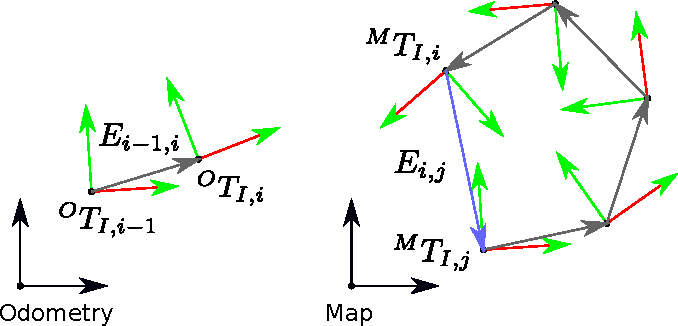
\includegraphics[width=0.5\textwidth]{../figs/graph_slam_residuals.pdf}
  \caption{Residuals used in pose graph optimization.}
  \label{fig:graph_slam_residuals}
\end{figure}
















\section{Pose Graph Optimization}

\subsection{Cost Function}

To analyze pose graph optimization, we begin by considering the residual vectors defined within the pose graph.
As shown in equations~(\ref{eq:odometry_edge}) and~(\ref{eq:loop_edge}), edges in the pose graph are defined as relative poses between two nodes.
Assuming these edges represent observations (i.e., fixed values), the following residual vector can be defined.
%
\begin{align}
  {\bf r}_{i, j}({}^{M}T_{I, i}, {}^{M}T_{I, j}) = \left( \log \left( E_{i, j}^{-1} {}^{M}T_{I, i}^{-1} {}^{M}T_{I, j} \right) \right)^{\vee}.
  \label{eq:pose_graph_residual}
\end{align}
%
Since equation~(\ref{eq:pose_graph_residual}) defines the residual vector for the edge between nodes $i$ and $j$, pose graph optimization is performed by finding the set of poses that minimizes the sum of these residuals.
%
\begin{align}
 E \left( \mathcal{T} \right) = \sum_{ i, j \in \mathcal{E} } \rho \left( \left\| {\bf r}_{i, j} \right\|_{ \Omega_{i, j} }^{2} \right),
  \label{eq:pose_graph_cost_function}
\end{align}
%
where $\left\| {\bf r}_{i, j} \right\|_{ \Omega_{i, j} }^{2} = {\bf r}_{i, j}^{\top} \Omega_{i, j} {\bf r}_{i, j}$ represents the squared Mahalanobis distance using the information matrix $\Omega_{i, j}$.





\subsection{Computation of the Jacobian}

To minimize the cost function in equation~(\ref{eq:pose_graph_cost_function}), we compute the Jacobians of the residual vector in equation~(\ref{eq:pose_graph_residual}) with respect to ${}^{M}T_{I, i}$ and ${}^{M}T_{I, j}$.
For this purpose, we introduce $\Delta_{i, j} = E_{i, j}^{-1} {}^{M}T_{I, i}^{-1} {}^{M}T_{I, j}$.
Using $\Delta_{i, j}$, the Jacobians can be derived by applying the chain rule as follows.
%
\begin{align}
  \begin{split}
    & \frac{ \partial {\bf r}_{i, j} }{ \partial {}^{M}T_{I, i} }
    = \frac{ \partial {\bf r}_{i, j} }{ \partial \Delta_{i, j} }
      \frac{ \partial \Delta_{i, j} }{ \partial {}^{M}T_{I, i} }, \\
%
    & \frac{ \partial {\bf r}_{i, j} }{ \partial {}^{M}T_{I, j} }
    = \frac{ \partial {\bf r}_{i, j} }{ \partial \Delta_{i, j} }
      \frac{ \partial \Delta_{i, j} }{ \partial {}^{M}T_{I, j} }.
  \end{split}
\end{align}
%
In the following, we consider each derivative separately.

First, let us compute $\partial {\bf r}_{i, j} / \partial \Delta_{i, j}$.
From equation~(\ref{eq:pose_graph_residual}), we need to find $J$ that satisfies the following relation.
%
\begin{align}
  \left( \log \left( \exp \left( \delta \boldsymbol \xi^{\wedge} \right) \Delta_{i, j} \right) \right)^{\vee} - \left( \log \left( \Delta_{i, j} \right) \right)^{\vee} = J \delta \boldsymbol \xi.
  \label{eq:deij_dDeltaij_J_deltaxi}
\end{align}
%
Here, $\log \left( \exp \left( \delta \boldsymbol \xi^{\wedge} \right) \Delta_{i, j} \right)^{\vee}$ can be approximated to first order using the BCH expansion as follows.
%
\begin{align}
  \left( \log \left( \exp \left( \delta \boldsymbol \xi^{\wedge} \right) \Delta_{i, j} \right) \right)^{\vee}
  \simeq {\bf r}_{i, j} + J_{l}^{-1} \left( {\bf r}_{i, j} \right) \delta \boldsymbol \xi,
  \label{eq:bch_1_order_approx}
\end{align}
%
where ${\bf r}_{i, j} = \left( \log \left( \Delta_{i, j} \right) \right)^{\vee}$, and $J_{l}(\cdot)$ is referred to as the left Jacobian of ${\rm SE}(3)$, defined as follows.
%
\begin{align}
  \begin{gathered}
    J_{l}( \boldsymbol \xi )
    = \left( \begin{matrix}
        J_{l}( \boldsymbol \phi ) & 0_{3 \times 3} \\
        Q( \boldsymbol \xi )      & J_{l}( \boldsymbol \phi ) \\
      \end{matrix} \right) \\
%
    J_{l}( \boldsymbol \phi ) = I_{3}
                              + \frac{ 1 - \cos \theta }{ \| \theta \|^{2} } \boldsymbol \phi^{\wedge}
                              + \frac{ \theta - \sin \theta }{ \| \theta \|^{3} } \left( \boldsymbol \phi^{\wedge} \right)^{2} \\
%
    Q( \boldsymbol \xi ) = \frac{1}{2} {\bf v}^{\wedge}
                         + \frac{1 - \alpha}{ \|\boldsymbol \phi \|^{2} } \left( \boldsymbol \phi^{\wedge} {\bf v}^{\wedge} + {\bf v}^{\wedge} \boldsymbol \phi^{\wedge} \right)
                         + \frac{\beta - 1}{ \|\boldsymbol \phi \|^{4} } \boldsymbol \phi^{\wedge} {\bf v}^{\wedge} \boldsymbol \phi^{\wedge} \\
%
    \alpha = \frac{ \sin \theta }{ \theta } \cdot \frac{ \theta + \sin \theta }{ 2 \left( 1 - \cos \theta \right) } \\
%
    \beta = \frac{1}{ \theta^{2} } \left( 1 - \frac{ \sin \theta }{ \theta } \right),
  \end{gathered}
  \label{eq:left_jacobian_se3}
\end{align}
%
where $\boldsymbol \xi^{\wedge} = \left( \left( {\bf v}^{\top} ~ \boldsymbol \phi^{\top} \right)^{\top} \right)^{\wedge} \in \mathfrak{se}(3)$, $\boldsymbol \phi^{\wedge} \in \mathfrak{so}(3)$, and $\theta = \| \boldsymbol \phi \|_{2}$\footnote{Equation (\ref{eq:left_jacobian_se3}) includes both the left Jacobians of ${\rm SE}(3)$ and ${\rm SO}(3)$. They are distinguished by whether the argument lies in $\mathfrak{se}(3)$ or $\mathfrak{so}(3)$.}.

From equations~(\ref{eq:deij_dDeltaij_J_deltaxi}) and~(\ref{eq:bch_1_order_approx}), $\partial {\bf r}_{i, j} / \partial \Delta_{i, j}$ is given as follows.
%
\begin{align}
  \frac{ \partial {\bf r}_{i, j} }{ \partial \Delta_{i, j} } = J_{l}^{-1}( {\bf r}_{i, j} )
  \label{eq:deij_dDeltaij}
\end{align}
%

Next, to compute the derivative $\partial \Delta_{i, j} / \partial {}^{M}T_{I, i}$, we first introduce
$\Delta_{i, j} \left( \delta \boldsymbol \xi \right) = E_{i, j}^{-1} \left( \exp \left( \delta \boldsymbol \xi^{\wedge} \right) {}^{M}T_{I, i} \right)^{-1} {}^{M}T_{I, j}$, where $\delta \boldsymbol \xi^{\wedge} \in \mathfrak{se}(3)$.
By multiplying $\Delta_{i, j} \left( \delta \boldsymbol \xi \right)$ from the left with $\Delta_{i, j}^{-1}$, we consider the variation around the identity element $I_{4}$.
%
\begin{align}
  \begin{split}
    \Delta_{i, j}^{-1} \Delta_{i, j} \left( \delta \boldsymbol \xi \right)
%
    = & {}^{M}T_{I, j}^{-1} {}^{M}T_{I, i} E_{i, j} E_{i, j}^{-1} {}^{M}T_{I, i}^{-1} \exp \left( -\delta \boldsymbol \xi^{\wedge} \right) {}^{M}T_{I, j}, \\
%
    = & {}^{M}T_{I, j}^{-1} \exp \left( -\delta \boldsymbol \xi \right) {}^{M}T_{I, j}, \\
%
    = & \exp \left( \left( -\operatorname{Ad}_{ {}^{M}T_{I, j}^{-1} } \delta \boldsymbol \xi \right)^{\wedge} \right), \\
    \simeq & I_{4} + \left( -\operatorname{Ad}_{ {}^{M}T_{I, j}^{-1} } \delta \boldsymbol \xi \right)^{\wedge}.
%
  \end{split}
\end{align}
%
By comparing with equation~(\ref{eq:dT_dT}), it follows that $\partial \Delta_{i, j} / \partial {}^{M}T_{I, i}$ is given by:
%
\begin{align}
  \frac{ \partial \Delta_{i, j} }{ \partial {}^{M}T_{I, i} } = - \operatorname{Ad}_{ {}^{M}T_{I, j}^{-1} }.
  \label{eq:dDeltaij_dTi}
\end{align}
%

From equations~(\ref{eq:deij_dDeltaij}) and~(\ref{eq:dDeltaij_dTi}), it follows that $\partial {\bf r}_{i, j} / \partial {}^{M}T_{I, i}$ is given by:
%
\begin{align}
  \frac{ \partial {\bf r}_{i, j} }{ \partial {}^{M}T_{I, i} } = -J_{l}^{-1}( {\bf r}_{i, j} ) \operatorname{Ad}_{ {}^{M}T_{I, j}^{-1} }.
  \label{eq:deij_dTi}
\end{align}
%
Similarly, by performing the same derivation, $\partial {\bf r}_{i, j} / \partial {}^{M}T_{I, j}$ can be obtained as follows:
%
\begin{align}
  \frac{ \partial {\bf r}_{i, j} }{ \partial {}^{M}T_{I, j} } = J_{l}^{-1}( {\bf r}_{i, j} ) \operatorname{Ad}_{ {}^{M}T_{I, i} }.
  \label{eq:deij_dTj}
\end{align}



\subsection{Optimization with the Gauss-Newton Method}

To minimize the cost function shown in equation~(\ref{eq:pose_graph_cost_function}), we employ the Gauss-Newton method.
First, the Jacobians of the residual vector ${\bf r}_{i, j}$ in equation~(\ref{eq:pose_graph_residual}) with respect to ${}^{M}T_{I, i}$ and ${}^{M}T_{I, j}$ are given by equations~(\ref{eq:deij_dTi}) and~(\ref{eq:deij_dTj}), respectively.
Let us denote these Jacobians as $J_{i}$ and $J_{j}$.
Now, the Jacobian of the residual vector ${\bf r}_{i, j}$ corresponding to the $i$-th and $j$-th edge is expressed as
$J_{i, j} = \left( 0 ~ \cdots ~ 0 ~ J_{i} ~ 0 ~ \cdots ~ 0 ~ J_{j} ~ 0 ~ \cdots ~ 0 \right) \in \mathbb{R}^{6 \times 6N}$,
since only the $i$-th and $j$-th poses affect the residual, and all other entries are zero.
Using this, we can compute the Hessian matrix $H \in \mathbb{R}^{6N \times 6N}$ and the gradient vector ${\bf b} \in \mathbb{R}^{6N}$.
%
\begin{align}
  \begin{gathered}
    H = \sum_{ ij \in \mathcal{E} } w_{i, j} J_{i, j}^{\top} J_{i, j}, \\
    {\bf b} = \sum_{ ij \in \mathcal{E} } w_{i, j} J_{i, j}^{\top} {\bf r}_{i, j}, \\
  \end{gathered}
  \label{eq:graph_slam_hessian_gradient}
\end{align}
%
where $w_{i, j} = \rho^{\prime} \left( \| {\bf r}_{i, j} \|_{ \Omega_{i, j} }^{2} \right)$.
Using this Hessian matrix and gradient, we solve for $\delta \boldsymbol \xi$ such that $H \delta \boldsymbol \xi = -{\bf b}$.
The vector $\delta \boldsymbol \xi \in \mathbb{R}^{6N}$ is composed of $N$ blocks, each corresponding to the update for one pose.
That is, if the $i$-th block is denoted as $\delta \boldsymbol \xi_{i} \in \mathbb{R}^{6}$, then the corresponding $i$-th pose ${}^{M}T_{I, i}$ is updated as follows:
%
\begin{align}
  {}^{M}T_{I, i} \leftarrow \exp \left( \delta \boldsymbol \xi_{i}^{\wedge} \right) {}^{M}T_{I, i}.
\end{align}
%

When implementing graph-based SLAM, the Hessian matrix has a size of $6N \times 6N$, and directly computing its inverse would be computationally very expensive.
However, in most cases, a typical graph-based SLAM problem results in $H$ being sparse, where most of the off-diagonal elements are zero.
Such a matrix is called a {\bf sparse matrix}, and by using dedicated solvers, it is possible to efficiently solve for $\delta \boldsymbol \xi$ in $H \delta \boldsymbol \xi = -{\bf b}$.
Therefore, in practice, instead of explicitly constructing a large Jacobian as in equation~(\ref{eq:graph_slam_hessian_gradient}), the computation is carried out by evaluating $J_{i}$ and $J_{j}$ and incrementally adding their contributions to the corresponding entries of the matrix.













\section{Loop Detection}
\label{subsec:gicp}

\subsection{Optimization of GICP}

As mentioned earlier, GICP is used for loop detection.
GICP is a method that can be applied to align two point clouds: the source point cloud $\mathcal{P}$ and the target point cloud $\mathcal{Q}$.
In GICP, each point cloud is represented using Gaussian distributions.
To achieve this, nearest-neighbor searches are first performed for all points in each point cloud to retrieve their neighboring points.
Using these neighboring points, the mean and covariance matrices are then computed.
The mean and covariance are calculated according to equations~(\ref{eq:points_mean}) and~(\ref{eq:points_covariance}).
Specifically, the $i$-th point of $\mathcal{P}$ is represented by $\bar{ {\bf p} }_{i}$ and $C_{i}^{p}$, while the $i$-th point of $\mathcal{Q}$ is represented by $\bar{ {\bf q} }_{i}$ and $C_{i}^{q}$.
Based on these, the cost function in GICP is defined as follows.
%
\begin{align}
  E \left( T \right) = \sum_{i=1}^{N} \rho \left( \left( \bar{ {\bf q} }_{i} - T \bar{ {\bf p} }_{i} \right)^{\top} \left( \hat{C}_{i}^{q} + T \hat{C}_{i}^{p} T^{-1} \right)^{-1} \left( \bar{ {\bf q} }_{i} - T \bar{ {\bf p} }_{i} \right) \right),
  \label{eq:gicp_cost_function}
\end{align}
%
where $\hat{C}^{p}$ and $\hat{C}^{q}$ are defined as follows.
%
\begin{align}
  \begin{gathered}
    \hat{C}^{p} = \left( \begin{matrix}
      C^{p}          & {\bf 0} \\
      {\bf 0}^{\top} & 0
    \end{matrix} \right) \in \mathbb{R}^{4 \times 4}, \\
%
    \hat{C}^{q} = \left( \begin{matrix}
      C^{q}          & {\bf 0} \\
      {\bf 0}^{\top} & 0
    \end{matrix} \right) \in \mathbb{R}^{4 \times 4}.
  \end{gathered}
\end{align}
%
Figure~\ref{fig:gicp_residual} illustrates the relationship of the residual used in GICP.

\begin{figure}[!t]
  \centering
  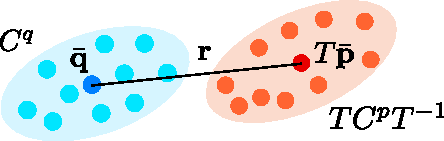
\includegraphics[width=0.3\textwidth]{../figs/gicp_residual.pdf}
  \caption{Residual error used in GICP.}
  \label{fig:gicp_residual}
\end{figure}

In this book, GICP is also solved using the Gauss-Newton method.
For notational simplicity, let ${\bf r}_{i} = \bar{ {\bf q} }_{i} - T \bar{ {\bf p} }_{i}$ and $\Omega_{i} = \left( \hat{C}_{i}^{q} + T \hat{C}_{i}^{p} T^{\top} \right)^{-1}$.
First, to compute the Jacobian of ${\bf r}_{i}$ with respect to $T$, we seek $J_{i}$ such that the following holds.
%
\begin{align}
  \bar{ {\bf q} }_{i} - \exp \left( \delta \boldsymbol \xi^{\wedge} \right) T \bar{ {\bf p} }_{i} - \left( \bar{ {\bf q} }_{i} - T \bar{ {\bf p} }_{i} \right) = J_{i} \delta \boldsymbol \xi.
  \label{eq:gicp_jacobi_approx}
\end{align}
%
Expanding the left-hand side of equation~(\ref{eq:gicp_jacobi_approx}) yields the following.
%
\begin{align}
  \begin{split}
    -\exp \left( \delta \boldsymbol \xi^{\wedge} \right) T \bar{ {\bf p} }_{i} + T \bar{ {\bf p} }_{i}
%
    = & - \left( \exp \left( \delta \boldsymbol \xi^{\wedge} \right) - I_{4} \right) T \bar{ {\bf p} }_{i}, \\
%
    = & - \left( \begin{matrix}
            \delta \boldsymbol \phi^{\wedge} & \delta {\bf v} \\
            {\bf 0}^{\top}                   & 0
          \end{matrix} \right)
          \left( \begin{matrix}
            \bar{ {\bf p} }_{i}^{'} \\
            1
          \end{matrix} \right), \\
%
    = & - \left( \begin{matrix}
            - \left( \bar{ {\bf p} }_{i}^{'} \right)^{\wedge} \delta \boldsymbol \phi + \delta {\bf v} \\
            0
          \end{matrix} \right), \\
%
    = & \left( \begin{matrix}
          -I_{3}         & \left( \bar{ {\bf p} }_{i}^{'} \right)^{\wedge} \\
          {\bf 0}^{\top} & {\bf 0}^{\top}
        \end{matrix} \right) \delta \boldsymbol \xi, \\
  \end{split}
\end{align}
%
where $\bar{ {\bf p} }_{i}^{'} = R \bar{ {\bf p} }_{i} + {\bf t}$.
Therefore, the $J_{i}$ that satisfies equation~(\ref{eq:gicp_jacobi_approx}) is given as follows.
%
\begin{align}
  J_{i} = \left( \begin{matrix}
            -I_{3}         & \left( \bar{ {\bf p} }_{i}^{'} \right)^{\wedge} \\
            {\bf 0}^{\top} & {\bf 0}^{\top}
          \end{matrix} \right).
  \label{eq:gicp_jacobian}
\end{align}
%
Using this Jacobian, the Hessian and gradient can be computed as follows.
%
\begin{align}
  \begin{gathered}
    H = \sum_{i=1} w_{i} J_{i}^{\top} \Omega_{i} J_{i}, \\
    {\bf b} = \sum_{i=1} w_{i} J_{i}^{\top} \Omega_{i} {\bf r}_{i}, \\
  \end{gathered}
  \label{eq:gicp_hessian_and_gradient}
\end{align}
%
where $w_{i} = \rho^{\prime} \left( {\bf r}_{i}^{\top} \Omega_{i} {\bf r}_{i} \right)$.
Using $H$ and ${\bf b}$, we solve for $\delta \boldsymbol \xi$ such that $H \delta \boldsymbol \xi = -{\bf b}$, and update the pose as $T \leftarrow \exp \left( \delta \boldsymbol \xi^{\wedge} \right) T$.

A brief note on the derivation of equation~(\ref{eq:gicp_hessian_and_gradient}): as discussed in Section~\ref{subsec:gauss-newton_method}, it is obtained by considering the cost function that uses the linear approximation of the residual vector when the state undergoes a small perturbation.
%
\begin{align}
  \sum_{i=1}^{N} \left( {\bf r}_{i} + J_{i} \delta \boldsymbol \xi \right)^{\top} \Omega_{i} \left( {\bf r}_{i} + J_{i} \delta \boldsymbol \xi \right)
  =
  \sum_{i=1}^{N} {\bf r}_{i}^{\top} \Omega_{i} {\bf r}_{i} + 2 \delta \boldsymbol \xi^{\top} \Omega_{i} J_{i} {\bf r}_{i} + \delta \boldsymbol \xi^{\top} J_{i}^{\top} \Omega_{i} J_{i} \delta \boldsymbol \xi,
\end{align}
%
Differentiating the right-hand side with respect to $\delta \boldsymbol \xi$ and setting it equal to 0 yields the following result (note that, compared to equation~(\ref{eq:gicp_hessian_and_gradient}), $w_{i}$ is omitted in the equation below).
%
\begin{align}
  \sum_{i=1}^{N} J_{i}^{\top} \Omega_{i} J_{i} \delta \boldsymbol \xi = -\sum_{i=1}^{N}  J_{i}^{\top} \Omega_{i} {\bf r}_{i}.
\end{align}
%



\subsection{Loop Detection Success Criteria}

To perform loop detection, GICP is used to minimize the cost function defined in equation~(\ref{eq:gicp_cost_function}), thereby aligning the point clouds.
Based on this alignment result, it is necessary to determine whether loop detection has succeeded or failed.
However, it is difficult to establish explicit criteria that reliably indicate the correctness of the alignment.
For instance, thresholds on the final value of the cost function or on the mean residual can serve as indicators to some extent, but they do not always provide a definitive judgment.
In practice, however, such indicators are often useful.
In the implementation presented in this book, thresholds are applied to the mean residual and to the alignment ratio (i.e., the proportion of points whose distance to the nearest neighbor is below a threshold).
These measures are then used to decide whether loop detection is deemed successful.

That said, this approach may still incorrectly classify failed alignments as successful.
If such erroneous information is incorporated into the graph, it may cause the optimization to diverge or fail.
For this reason, it is also effective to employ robust kernels, such as the Huber loss, in the graph optimization described in equation~(\ref{eq:graph_slam_hessian_gradient}).











\section{Computation of Coordinate Transformations and Map Construction}

\subsection{Transformations}

Using LIO, we obtain the IMU pose ${}^{O}T_{I}$ in the odometry frame.
When pose graph optimization is performed, the poses of newly detected keyframes are corrected, resulting in the IMU pose ${}^{M}T_{I}$ in the map frame.
To compute the transformation ${}^{M}T_{O}$ between the map and odometry frames, as illustrated in Figure~\ref{fig:map_odom_transformation}, we assume that the IMU pose in the map frame and the IMU pose in the odometry frame coincide.
From this relationship, ${}^{M}T_{O}$ can be obtained as follows.
%
\begin{align}
  \begin{split}
    {}^{M}T_{O} = & {}^{M}T_{I} {}^{O}T_{I}^{-1}, \\
                = & {}^{M}T_{I} {}^{I}T_{O}.
  \end{split}
\end{align}
%
Although the details are not discussed in this book, the transformation ${}^{M}T_{O}$ is obtained in the same manner when performing localization.

\begin{figure}[!t]
  \centering
  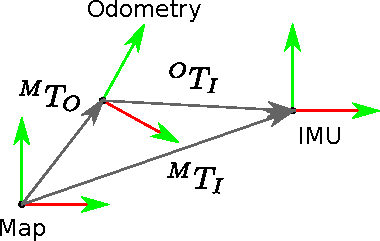
\includegraphics[width=0.3\textwidth]{../figs/map_odom_transformation.pdf}
  \caption{Residuals used in pose graph optimization.}
  \label{fig:map_odom_transformation}
\end{figure}



\subsection{Map Construction}

Once the pose graph optimization is completed, each keyframe in the map frame is corrected to ${}^{M}T_{I, i}$.
Using these poses together with the corresponding point clouds ${}^{I}\mathcal{P}_{i}$ for each keyframe, the point cloud map is constructed as follows.
%
\begin{align}
  {}^{M}\mathcal{M} = \bigcup_{i=1}^{K} \bigcup_{{}^{I}{\bf p} \in {}^{I}\mathcal{P}_{i}} {}^{M}T_{I, i} {}^{I}{\bf p},
\end{align}
%
where $K$ denotes the number of keyframes.
In the graph-based SLAM implementation presented in this book, however, this map point cloud is not directly used in the processing.
Therefore, it is sufficient to generate it only once at the end of the SLAM process.
That said, executing it after each pose graph optimization allows one to verify online whether the map is being correctly constructed.
For this reason, the implementation described in this book performs this operation after every optimization.










\section{Practical Considerations}

In the method presented in this chapter, keyframes are detected by applying a threshold on the amount of motion, and the LiDAR point cloud corresponding to each keyframe is stored.
A map is then constructed by transforming these point clouds according to their associated keyframe poses.
One drawback of this approach is that not all LiDAR point clouds are used in the mapping process, which results in a lower map density.
To increase the density, one could, for example, accumulate LiDAR scans over a fixed time interval and then detect a keyframe.
However, this approach causes memory usage to grow over time.
On the other hand, the motion-based keyframe detection method scales memory usage with motion rather than time, making it more memory-efficient.
Thus, there is a trade-off between density and memory cost.

If the sole goal is to create a denser point cloud map, one practical approach is to reuse the same dataset used for SLAM-based mapping, perform localization again on this map, and then remap the point clouds according to the refined poses.
While slightly more cumbersome, this method enables the creation of a high-density point cloud map without significant memory concerns.
However, it should be noted that the result will not necessarily guarantee globally consistent mapping, since it is not based on optimizing global alignment of the point cloud data.

The method introduced in this chapter falls under graph-based SLAM using a pose graph.
When using a pose graph, LiDAR point clouds are not directly optimized, and therefore, mapping accuracy may be lower compared to full graph-based SLAM.
In general graph-based SLAM, however, all LiDAR point clouds are rarely optimized due to memory constraints.
Instead, feature points or landmarks are extracted from the LiDAR point clouds and incorporated into the optimization.
Consequently, the quality of mapping depends heavily on the performance of feature/landmark detection and association.

With modern 3D LiDARs providing long-range measurements and high-density point clouds, even simple point cloud registration between two scans can achieve highly accurate relative pose estimates.
Therefore, under such conditions, pose graph optimization alone is often sufficient to generate an accurate map.
Nonetheless, as demonstrated in works such as \cite{KoideRAS2024}, incorporating full map optimization can further improve accuracy, meaning whether pose graph optimization alone is sufficient depends on the use case.

In the method described here, loop detection is performed simply by applying scan matching between nearby keyframes.
As mentioned in Section~\ref{sec:scan_matching_実用にあたって}, one of the prerequisites for successful scan matching is having a sufficiently accurate initial pose.
However, odometry inherently accumulates drift error, and as the trajectory grows longer during SLAM execution, the accuracy of initial poses used for loop detection scan matching decreases.
Thus, relying solely on scan matching may fail to close large loops.
In such cases, alternative approaches such as extracting features or descriptors from LiDAR scans and detecting similar scans based on these features are required.
However, such methods generally tend to be less accurate than loop detection based purely on scan matching.
Therefore, additional considerations such as outlier detection during pose graph optimization become important.

Even when loop detection relies solely on scan matching, correctly closing loops effectively compensates for accumulated odometry drift.
From a practical standpoint, designing trajectories that facilitate loop closures is often a strategy to ensure successful map building.
However, when loops are too large, the system may reach its performance limits, and incorporating alternative approaches becomes necessary.


